\documentclass[12pt,a4paper]{article}

% ==================== PAQUETES ====================
\usepackage[utf8]{inputenc}
\usepackage[T1]{fontenc}
\usepackage[spanish,es-tabla]{babel}
\usepackage{mathpazo}            % Palatino
\usepackage[scaled=.95]{couriers}

% Márgenes
\usepackage[top=2.5cm, bottom=2.5cm, left=3cm, right=2.5cm, headheight=13.6pt]{geometry}

% Portada
\usepackage{titling}
\usepackage{abstract}

% Header / Footer
\usepackage{fancyhdr}
\pagestyle{fancy}
\fancyhf{}
\fancyhead[L]{\small\itshape Del sistema experto al Context Graph}
\fancyhead[R]{\small\thepage}
\renewcommand{\headrulewidth}{0.4pt}

% Figuras, tablas, captions
\usepackage{graphicx}
\usepackage{float}
\usepackage{caption}
\usepackage[table,xcdraw]{xcolor}
\usepackage{booktabs}
\usepackage{longtable}

% Matemáticas
\usepackage{amsmath}
\usepackage{amssymb}

% Diagramas TikZ
\usepackage{tikz}
\usetikzlibrary{shapes,arrows,positioning,fit,backgrounds,calc}
\tikzset{phase/.style={draw, fill=blue!8, rounded corners, minimum height=1.0cm, minimum width=2.5cm, align=center, font=\small\bfseries, inner sep=4pt}}
\tikzset{arrow/.style={->, thick, color=blue!60!black}}

% Código
\usepackage{listings}
\usepackage{xcolor}

\lstset{
  basicstyle=\small\ttfamily,
  backgroundcolor=\color{gray!5},
  frame=single,
  rulecolor=\color{gray!30},
  breaklines=true,
  tabsize=2,
  numbers=left,
  numberstyle=\tiny\color{gray},
  captionpos=b,
  inputencoding=utf8,
  literate={á}{{\'a}}1 {é}{{\'e}}1 {í}{{\'i}}1 {ó}{{\'o}}1 {ú}{{\'u}}1
           {ñ}{{\~n}}1 {Á}{{\'A}}1 {É}{{\'E}}1 {Í}{{\'I}}1 {Ó}{{\'O}}1
           {Ú}{{\'U}}1 {Ñ}{{\~N}}1 {º}{{\textdegree}}1,
}

% Hipervínculos
\usepackage[colorlinks=true, citecolor=blue, linkcolor=blue, urlcolor=blue]{hyperref}

% ==================== METADATOS ====================
\title{Del sistema experto al Context Graph:\\Un enfoque basado en grafos de conocimiento\\para la consulta auditable de datos políticos}
\author{Proyecto 8 --- Big Data e Inteligencia Artificial}
\date{13 de mayo de 2026}

% ==================== DOCUMENTO ====================
\begin{document}

% ---------------- PORTADA ----------------
\begin{titlepage}
\centering
\vspace*{2cm}

{\LARGE\bfseries Del sistema experto al Context Graph\par}
\vspace{0.3cm}
{\Large Un enfoque basado en grafos de conocimiento\\para la consulta auditable de datos políticos\par}

\vspace{1.5cm}

{\large\textbf{Proyecto 8} --- Big Data e Inteligencia Artificial\par}

\vspace{0.5cm}
{\large 13 de mayo de 2026}

\vspace{3cm}

\begin{abstract}
Este proyecto presenta la evolución de los sistemas expertos clásicos hacia los \textit{Context Graphs}, una arquitectura que combina grafos de conocimiento (\textit{Knowledge Graphs}) con metadatos de procedencia y vigencia temporal. Sobre el dominio de la política española (XV legislatura y Tercer Gobierno Sánchez), se implementa un pipeline completo: \textit{scraping} de fuentes estructuradas (Wikipedia) mediante \texttt{r.jina.ai}, extracción de tripletes semánticos vía LLM (Cerebras + Llama 3.1~8B), construcción de un grafo dirigido con \texttt{networkx} (715 nodos, 812 aristas), y un motor de preguntas y respuestas (\textit{QA}) con trazabilidad total a la fuente y fecha de extracción. Los resultados demuestran que un Context Graph permite respuestas auditables y libres de alucinaciones, superando las limitaciones de los sistemas RAG vectoriales en dominios con datos temporales y relaciones complejas.
\end{abstract}
\end{titlepage}

% ---------------- SUMARIO ----------------
\tableofcontents
\newpage

% ==================== 1. INTRODUCCIÓN ====================
\section{Introducción}
\label{sec:intro}

Los sistemas expertos clásicos, surgidos en la d\'ecada de 1970, se fundamentan en tres componentes esenciales: una \textbf{base de conocimiento} que almacena hechos y reglas del dominio, un \textbf{motor de inferencia} que aplica esas reglas para deducir nuevos hechos, y una \textbf{interfaz de usuario} que permite la interacci\'on \cite{hogan2021kg}. Su din\'amica de funcionamiento sigue un ciclo iterativo: el motor de inferencia examina las reglas, selecciona aquellas cuyas premisas se cumplen, ejecuta la acci\'on correspondiente y a\~nade los nuevos hechos a la base, repitiendo el proceso hasta alcanzar una conclusi\'on o agotar las reglas aplicables.

Por ejemplo, en el dominio de la pol\'itica espa\~nola, una regla cl\'asica podr\'ia expresarse como:

\begin{quote}
\texttt{SI} \textit{persona} = ``Pedro S\'anchez'' \\
\texttt{Y} \textit{evento} = ``investidura'' \\
\texttt{Y} \textit{fecha} $\geq$ ``2023-11-16'' \\
\texttt{ENTONCES} \textit{cargo} = ``presidente del Gobierno''
\end{quote}

Este enfoque ofrece respuestas deterministas y completamente trazables, ya que cada conclusi\'on se justifica mediante la cadena de reglas aplicadas. Sin embargo, presenta limitaciones fundamentales: las reglas deben codificarse manualmente, lo que no escala a dominios con cientos de entidades y relaciones cambiantes; cualquier modificaci\'on normativa o pol\'itica requiere actualizar las reglas una a una; y el sistema carece de la flexibilidad del lenguaje natural para explicar sus conclusiones.

La evoluci\'on hacia los \textbf{grafos de conocimiento} (\textit{Knowledge Graphs}) supuso un avance cualitativo: en lugar de reglas r\'igidas, se modelan entidades, conceptos y relaciones de manera expl\'icita, formando una red sem\'antica navegable \cite{hogan2021kg}. Esta estructura aporta interoperabilidad y capacidad de razonamiento sobre relaciones complejas, pero sigue siendo est\'atica: los datos se incorporan en lotes y no conservan informaci\'on sobre su origen ni su vigencia temporal.

Con la llegada de los grandes modelos de lenguaje (\textit{LLMs}), surgi\'o la posibilidad de extraer conocimiento de texto no estructurado de forma autom\'atica \cite{pan2024kg}. Sin embargo, los LLMs introducen un problema grave: las \textbf{alucinaciones}, esto es, informaci\'on plausible pero factualmente incorrecta \cite{ji2023survey}. Los sistemas RAG (\textit{Retrieval-Augmented Generation}) mitigaron parcialmente este problema al recuperar fragmentos de documentos relevantes antes de generar la respuesta \cite{lewis2020rag}. Sin embargo, la recuperaci\'on vectorial opera sobre fragmentos de texto sin conciencia de las relaciones entre entidades, lo que limita su eficacia cuando los datos tienen una fuerte dimensi\'on temporal o requieren encadenar m\'ultiples hechos para llegar a una conclusi\'on.

El \textbf{Context Graph} surge como respuesta a estas limitaciones: un grafo de conocimiento que enriquece cada relaci\'on con metadatos de procedencia (URL de origen), vigencia temporal (\texttt{valido\_desde}, \texttt{valido\_hasta}) y confianza. De este modo, el LLM act\'ua como extractor sem\'antico flexible, mientras que el grafo proporciona una memoria verificable y trazable. Este enfoque ha sido reconocido por el W3C (grupo comunitario, febrero de 2026), Thoughtworks (Technology Radar vol.~34, abril de 2026) e IBM como capa de contexto para sistemas aumentados con LLM.

\subsection{Motivaci\'on}

El dominio de la política española es un caso de estudio ideal para demostrar estas limitaciones:
\begin{itemize}
  \item \textbf{Red compleja}: políticos, partidos, cargos, leyes y pactos forman una red densa de relaciones.
  \item \textbf{Componente temporal crítico}: los roles cambian con cada legislatura, los pactos se firman y caducan.
  \item \textbf{Necesidad de trazabilidad}: en contextos políticos, la fuente exacta y la fecha son tan importantes como la respuesta misma.
\end{itemize}
Los LLMs solos alucinan pactos, fechas y nombres. RAG vectorial recupera fragmentos pero no puede razonar sobre la cadena de relaciones entre entidades.

\subsection{Objetivos}

\begin{enumerate}
  \item Construir un \textbf{Context Graph}: un grafo de conocimiento donde cada arista almacena metadatos de procedencia (fuente URL), vigencia temporal (\texttt{valido\_desde}, \texttt{valido\_hasta}) y confianza.
  \item Implementar un \textbf{pipeline automatizado} de scraping, extracción semántica, construcción del grafo y consulta.
  \item Demostrar \textbf{3 consultas QA} con trazabilidad completa, incluyendo al menos una consulta \textit{multi-hop} que requiera recorrer múltiples nodos.
  \item Comparar el enfoque Context Graph con RAG vectorial, analizando ventajas y desventajas.
\end{enumerate}

% ==================== 2. ARQUITECTURA ====================
\section{Arquitectura del sistema}
\label{sec:arquitectura}

La arquitectura sigue un pipeline en cinco fases, ilustrado en la Figura~\ref{fig:arquitectura}:

\begin{figure}[H]
\centering
\begin{tikzpicture}[node distance=0.4cm and 0.6cm]
  % Columna izquierda: fases impares
  \node[phase] (scrape) {Scraping\\\footnotesize\texttt{r.jina.ai}};
  \node[phase, below=of scrape] (graph) {Context\\Graph\\\footnotesize\texttt{networkx}};
  \node[phase, below=of graph] (viz) {Visualización\\\footnotesize Graphviz};
  
  % Columna derecha: fases pares  
  \node[phase, right=4.5cm of scrape] (extract) {Extracción\\\footnotesize Cerebras + LLM};
  \node[phase, right=4.5cm of graph] (qa) {QA\\\footnotesize Consultas trazables};
  
  % Etiquetas de contexto en el medio
  \node[align=center, font=\scriptsize\itshape, text=gray!60!black] at ($(scrape)!0.5!(extract) + (0,0.6)$) {Wikipedia};
  \node[align=center, font=\scriptsize\itshape, text=gray!60!black] at ($(scrape)!0.5!(extract) + (0,-0.6)$) {Markdown};
  \node[align=center, font=\scriptsize\itshape, text=gray!60!black] at ($(graph)!0.5!(qa) + (0,0.5)$) {Tripletes\\JSON};
  \node[align=center, font=\scriptsize\itshape, text=gray!60!black] at ($(graph)!0.5!(qa) + (0,-0.7)$) {Grafo\\dirigido};
  
  % Flechas pipeline principal
  \draw[arrow] (scrape.east) -- node[above, font=\tiny] {texto plano} (extract.west);
  \draw[arrow] (extract.south) |- node[right, font=\tiny, pos=0.4] {tripletes} (qa.east);
  \draw[arrow] (scrape.south) -- node[left, font=\tiny] {datos} (graph.north);
  \draw[arrow] (graph.south) -- node[left, font=\tiny] {archivo .dot} (viz.north);
  \draw[arrow] ($(graph.east) + (0,0.2)$) -- node[above, font=\tiny] {carga} ($(qa.west) + (0,0.2)$);
  \draw[arrow] (qa.west) -- node[below, font=\tiny] {consulta} ($(graph.east) - (0,0.2)$);
  
  % Caja general
  \begin{pgfonlayer}{background}
    \node[draw, dashed, gray!30, rounded corners, fit={(scrape.north-|scrape.west) (viz.south-|qa.east)}, inner xsep=12pt, inner ysep=10pt, label={[gray, font=\footnotesize\bfseries]north:Pipeline completo}] {};
  \end{pgfonlayer}
\end{tikzpicture}
\caption{Arquitectura general del sistema en cinco fases. Las flechas sólidas indican el flujo principal de datos; la flecha bidireccional entre Context Graph y QA representa el ciclo consulta-respuesta.}
\label{fig:arquitectura}
\end{figure}

\subsection{Fuentes de datos}

Se seleccionaron dos páginas de Wikipedia por su riqueza en fechas, relaciones y entidades políticas:

\begin{itemize}
  \item \href{https://es.wikipedia.org/wiki/XV_legislatura_de_Espa%C3%B1a}{XV legislatura de España} --- composición del Congreso, pactos de investidura, cronología de eventos.
  \item \href{https://es.wikipedia.org/wiki/Tercer_Gobierno_S%C3%A1nchez}{Tercer Gobierno Sánchez} --- ministerios, nombramientos, carteras.
\end{itemize}

% ==================== 3. IMPLEMENTACIÓN ====================
\section{Implementación}
\label{sec:implementacion}

\subsection{Scraping (\texttt{scrape.py})}

El scraping se realiza mediante la API de \texttt{r.jina.ai}, que convierte páginas web a Markdown limpio. Se implementó codificación URL para caracteres especiales (ñ, tildes):

\begin{lstlisting}[caption={scrape.py --- extracción de contenido a Markdown}, label={lst:scrape}]
URLS = [
    "https://es.wikipedia.org/wiki/XV_legislatura_de_España",
    "https://es.wikipedia.org/wiki/Tercer_Gobierno_Sánchez"
]

def fetch_markdown(url):
    parsed_url = urllib.parse.urlparse(url)
    encoded_path = urllib.parse.quote(parsed_url.path)
    safe_url = urllib.parse.urlunparse(
        (parsed_url.scheme, parsed_url.netloc, encoded_path,
         parsed_url.params, parsed_url.query, parsed_url.fragment)
    )
    req = urllib.request.Request(API_BASE + safe_url,
                                 headers={"User-Agent": "Mozilla/5.0"})
    with urllib.request.urlopen(req) as response:
        return response.read().decode('utf-8')
\end{lstlisting}

El resultado son dos archivos Markdown con 273 líneas (\texttt{Tercer\_Gobierno\_Sánchez.md}) y 1238 líneas (\texttt{XV\_legislatura\_de\_España.md}), totalizando 1511 líneas de contenido semánticamente rico.

\subsection{Extracción de tripletes (\texttt{extract\_cerebras.py})}

La extracción semántica convierte texto no estructurado en tripletes \texttt{(sujeto, predicado, objeto)} con metadatos. Se utiliza el modelo Llama 3.1~8B a través de la API de Cerebras.

\subsubsection*{Chunking y solapamiento}

Los textos largos se dividen en fragmentos (\textit{chunks}) de 5200 caracteres con solapamiento de 450 caracteres para evitar perder contexto en los cortes:

\begin{lstlisting}[caption={Estrategia de chunking con solapamiento}, label={lst:chunking}]
def chunk_text(text, chunk_size=5200, overlap=450):
    chunks = []
    start = 0
    while start < len(text):
        end = min(start + chunk_size, len(text))
        chunks.append(text[start:end])
        if end >= len(text):
            break
        start = max(0, end - overlap)
    return chunks
\end{lstlisting}

\subsubsection*{Estructura del triplete}

Cada triplete extraído sigue un formato JSON con metadatos obligatorios:

\begin{lstlisting}[caption={Estructura de un triplete}, label={lst:triplete}]
{
    "sujeto": "Pedro Sánchez",
    "predicado": "fue investido",
    "objeto": "presidente del Gobierno",
    "fuente": "https://es.wikipedia.org/wiki/XV_legislatura_de_España",
    "fecha_extraccion": "2026-05-13",
    "valido_desde": "2023-11-16",
    "valido_hasta": null,
    "confianza": 1.0
}
\end{lstlisting}

La desduplicación se realiza por tupla \texttt{(sujeto, predicado, objeto, fuente)} para evitar tripletes repetidos entre \textit{chunks}.

\subsection{Construcción del grafo (\texttt{build\_graph.py})}

El grafo se construye con \texttt{networkx.DiGraph}. Cada triplete genera dos aristas:

\begin{enumerate}
  \item \texttt{fuente\_node --menciona--> sujeto} (metadatos: fuente, fecha)
  \item \texttt{sujeto --predicado--> objeto} (metadatos: predicado, fuente, fecha, validez)
\end{enumerate}

\begin{lstlisting}[caption={Construcción del grafo dirigido}, label={lst:graph}]
G = nx.DiGraph()
for item in load_triplets(filepath):
    G.add_node(sujeto)
    G.add_node(objeto)
    G.add_edge(source_node, sujeto, predicado="menciona",
               fuente=item["fuente"], fecha=item["fecha_extraccion"])
    G.add_edge(sujeto, objeto, predicado=predicado,
               fuente=item["fuente"], fecha=item["fecha_extraccion"])
\end{lstlisting}

El grafo resultante contiene \textbf{715 nodos} y \textbf{812 aristas}, con una densidad suficiente para consultas multi-hop complejas.

\subsection{Visualización (\texttt{build\_graph\_dot.py})}

Para obtener una representación legible del grafo en formato A4, se implementó un generador basado en \textbf{Graphviz}~\cite{graphviz}. El proceso consta de dos etapas:

\begin{enumerate}
  \item \textbf{Selección de hubs}: del grafo completo de 715 nodos, se extraen los 22 nodos más conectados (por grado de centralidad), preservando siempre los dos nodos fuente. Se filtran además nodos ruidosos (artefactos de la extracción LLM).
  \item \textbf{Renderizado con \texttt{neato}}: el subgrafo se exporta a formato DOT y se renderiza con el motor \texttt{neato} (distribución por muelles o \textit{spring model}), que minimiza el cruce de aristas y distribuye los nodos uniformemente. Se utiliza una resolución de 250~dpi con etiquetas de entre 9 y 14 puntos.
\end{enumerate}

Las reglas estéticas aplicadas son:

\begin{itemize}
  \item \textbf{Color dorado}: nodos fuente (documentos).
  \item \textbf{Color azul}: entidades políticas.
  \item \textbf{Aristas discontinuas}: relaciones ``menciona'' (fuente $\rightarrow$ entidad).
  \item \textbf{Aristas sólidas etiquetadas}: relaciones semánticas con el tipo de predicado.
\end{itemize}

La Figura~\ref{fig:graph} muestra el resultado.

\begin{figure}[p]
\centering
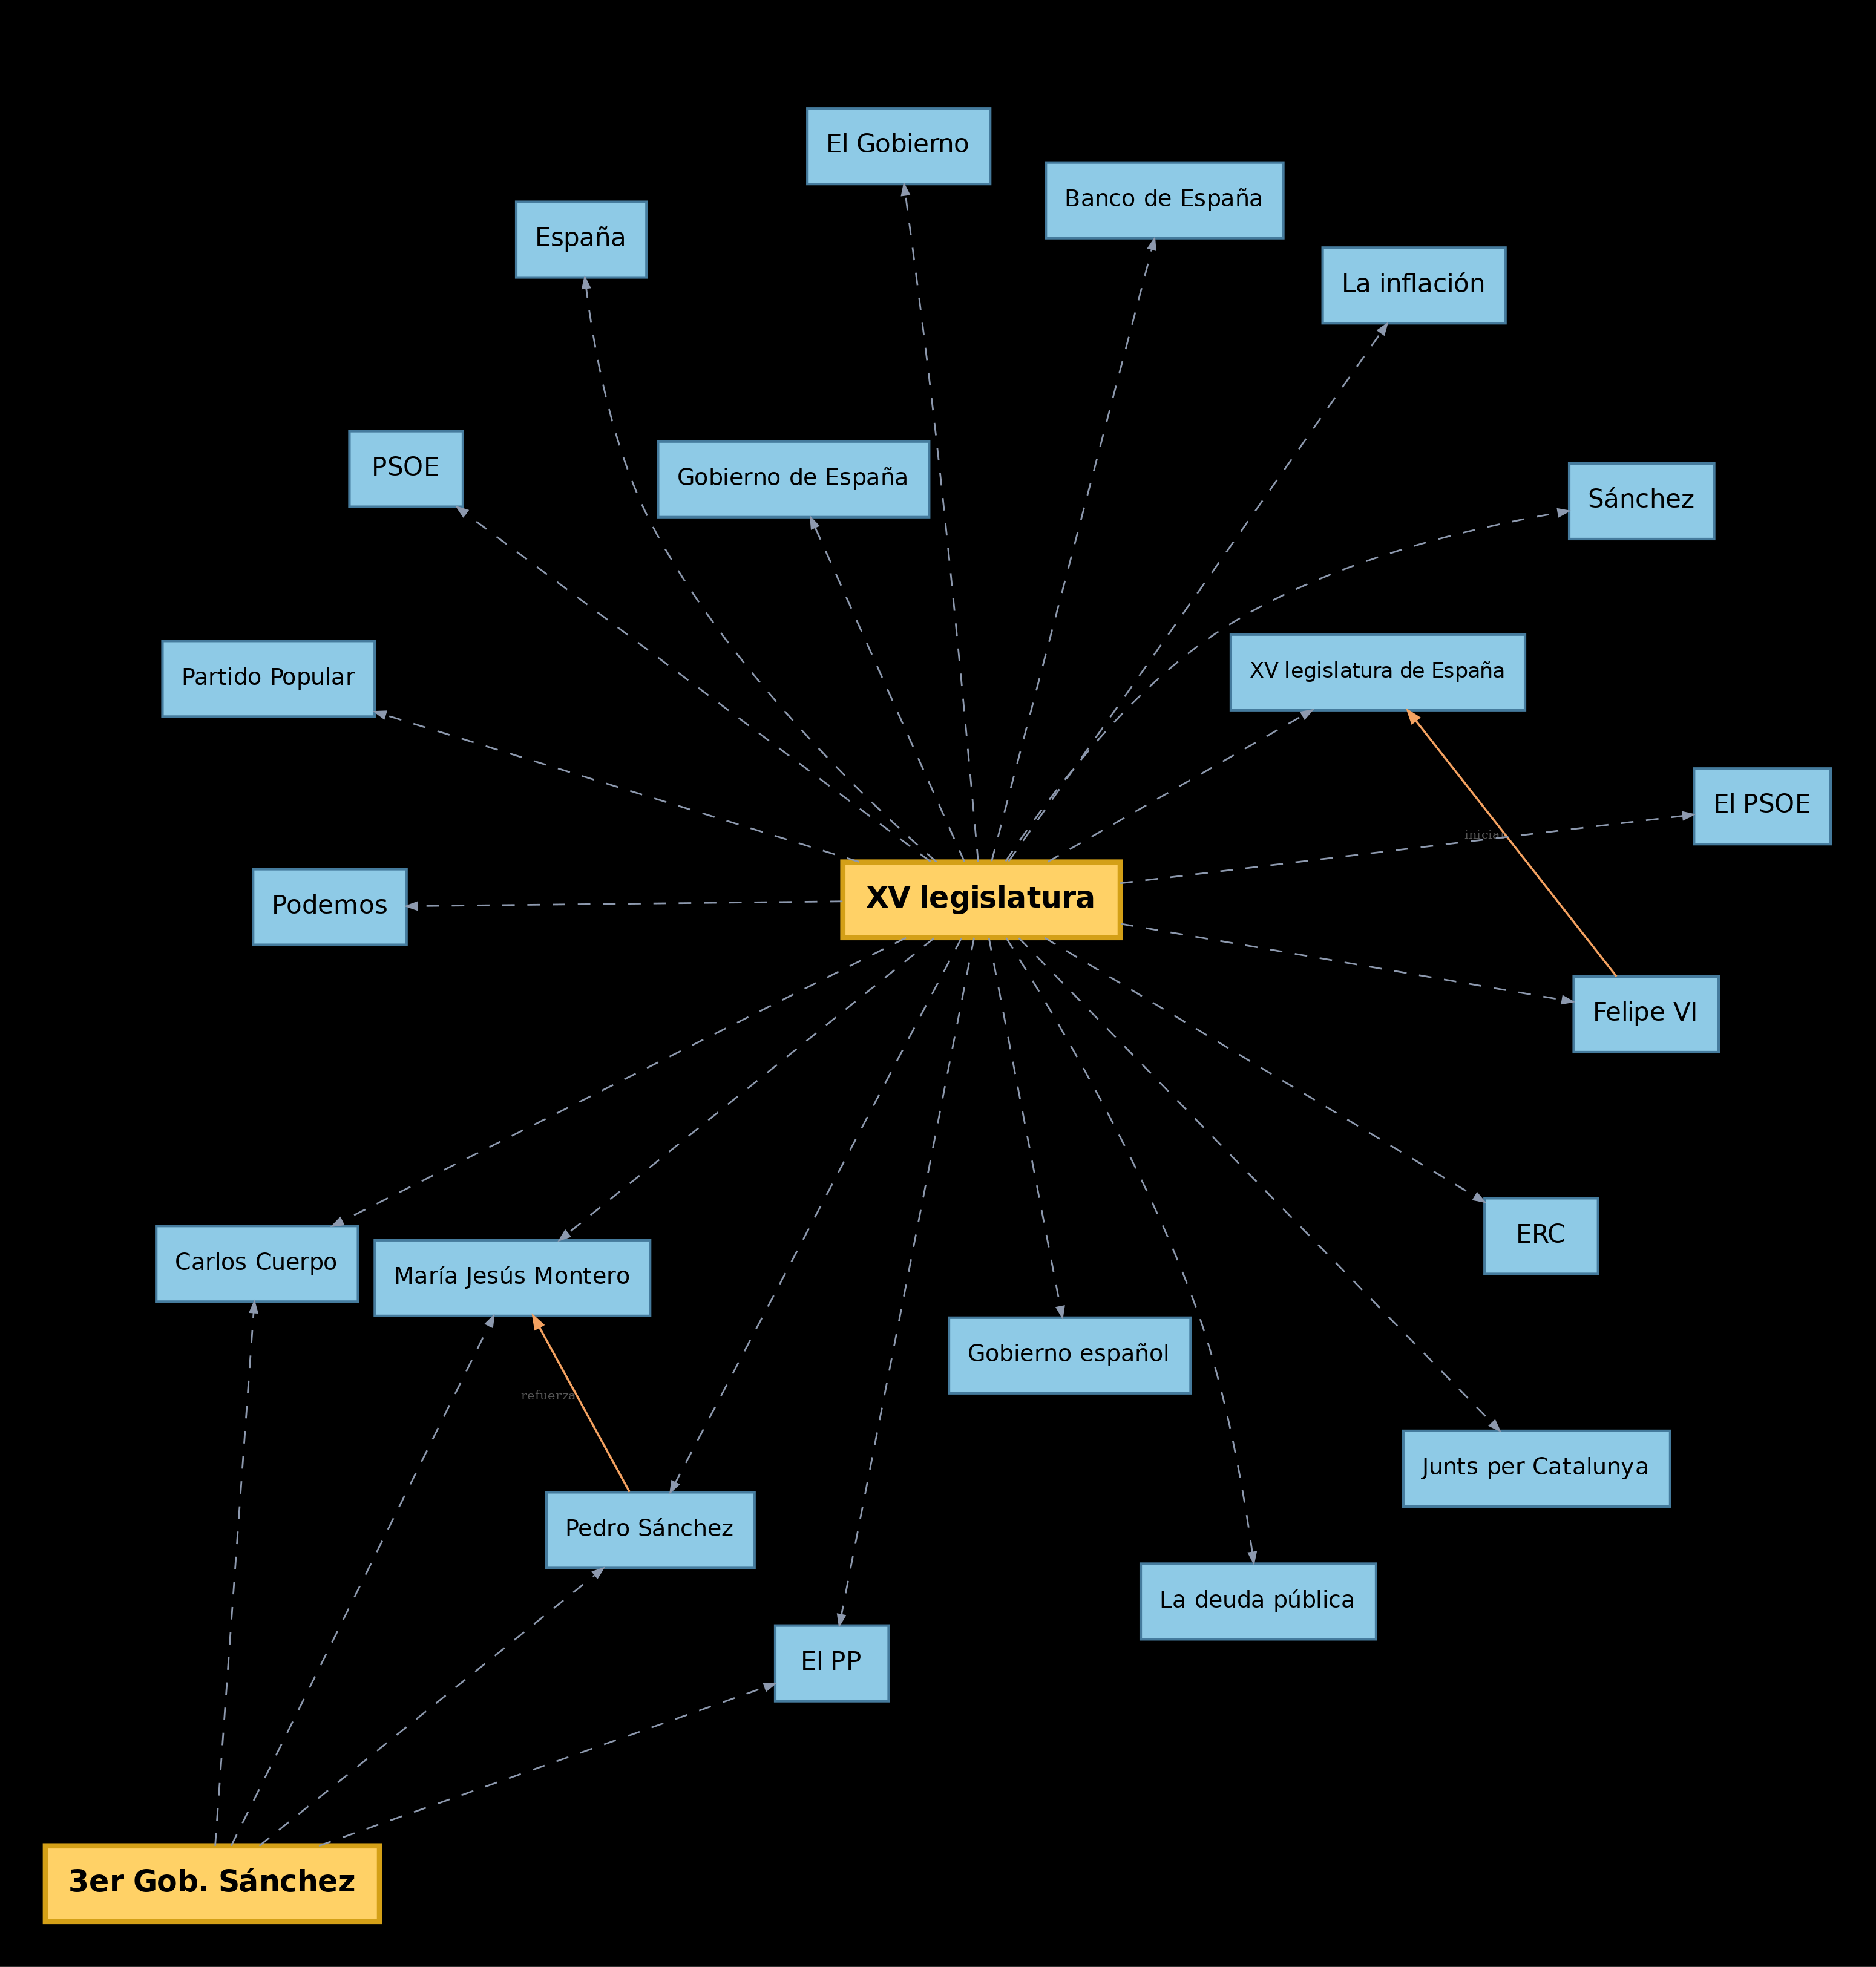
\includegraphics[width=\textwidth,height=\textheight,keepaspectratio]{graph.png}
\caption{Context Graph — 22 hubs más conectados del dominio de política española, renderizados con el motor \texttt{neato} (distribución por muelles). Los nodos dorados son las fuentes documentales; los azules son entidades políticas. Cada arista etiquetada indica el tipo de relación semántica.}
\label{fig:graph}
\end{figure}

\subsection{Motor de consultas (\texttt{qa\_graph.py})}

El motor de QA recorre el grafo dirigido construido por \texttt{build\_graph.py} para responder preguntas mediante dos estrategias:

\begin{enumerate}
  \item \textbf{Consultas directas}: buscan una arista con un predicado concreto desde un nodo origen (\texttt{answer\_direct}).
  \item \textbf{Consultas multi-hop}: emplean BFS (búsqueda en anchura) para encontrar caminos entre dos nodos (\texttt{find\_path}), permitiendo responder preguntas que requieren varios saltos de inferencia.
\end{enumerate}

\begin{lstlisting}[caption={qa\_graph.py --- funciones principales de consulta}, label={lst:qa}]
def answer_direct(graph, subject, predicate=None):
    """Respuesta directa: busca una arista desde 'subject'
       cuyo predicado coincida."""
    for _, target, edge in graph.out_edges(subject, data=True):
        if predicate is None or edge.get("predicado") == predicate:
            return target, edge
    return None, None

def find_path(graph, start, goal):
    """BFS para consultas multi-hop."""
    queue = deque([(start, [start])])
    visited = {start}
    while queue:
        node, path = queue.popleft()
        if node == goal:
            return path
        for neighbor in graph.successors(node):
            if neighbor in visited:
                continue
            visited.add(neighbor)
            queue.append((neighbor, path + [neighbor]))
    return None
\end{lstlisting}

Las consultas concretas y sus resultados se presentan en la Sección~\ref{sec:qa}.

% ==================== 4. RESULTADOS ====================
\section{Resultados: preguntas y respuestas}
\label{sec:qa}

El motor de QA (\texttt{qa\_graph.py}) implementa dos modos de consulta:

\begin{description}
  \item[Directa:] busca una arista específica \texttt{(sujeto, predicado)} y devuelve el objeto con sus metadatos.
  \item[Multi-hop:] realiza BFS (\textit{breadth-first search}) desde un nodo origen hasta un nodo destino, reconstruyendo la ruta completa.
\end{description}

\subsection{Consulta 1: directa}
\label{q1}

\begin{quote}
\textbf{Pregunta:} ¿Cuándo comenzó la XV legislatura de España?
\end{quote}

El sistema busca la arista \texttt{XV legislatura de España --comenzó--> ?} y obtiene:

\begin{lstlisting}
Respuesta: Comenzó el 17 de agosto de 2023
Fuente: https://es.wikipedia.org/wiki/XV_legislatura_de_España
Fecha de extracción: 2026-05-13
Validez: 2023-08-17 (continúa)
\end{lstlisting}

\subsection{Consulta 2: directa}
\label{q2}

\begin{quote}
\textbf{Pregunta:} ¿Quién fue investido presidente del Gobierno?
\end{quote}

\begin{lstlisting}
Respuesta: Pedro Sánchez
Fuente: https://es.wikipedia.org/wiki/XV_legislatura_de_España
Fecha de extracción: 2026-05-13
Validez: desde 2023-11-16
\end{lstlisting}

\subsection{Consulta 3: multi-hop}
\label{q3}

\begin{quote}
\textbf{Pregunta:} ¿Qué cargo se atribuye a Pedro Sánchez en la página del Tercer Gobierno de Pedro Sánchez?
\end{quote}

Esta consulta requiere recorrer dos aristas (multi-hop):

\begin{lstlisting}
Respuesta: presidente del Gobierno

Ruta:
1. Tercer Gobierno de Pedro Sánchez --menciona--> Pedro Sánchez
   Fuente: https://es.wikipedia.org/wiki/Tercer_Gobierno_Sánchez
2. Pedro Sánchez --ser--> investido presidente del Gobierno
   Fuente: https://es.wikipedia.org/wiki/XV_legislatura_de_España
\end{lstlisting}

La trazabilidad es completa: cada paso de la inferencia está respaldado por una fuente URL y una fecha de extracción. No hay ``caja negra''.

% ==================== 5. DISCUSIÓN ====================
\section{Discusión: Context Graph vs. RAG vectorial}
\label{sec:discusion}

La Tabla~\ref{tab:comparacion} resume las diferencias fundamentales entre ambos enfoques:

\begin{table}[H]
\centering
\caption{Comparación: Context Graph vs. RAG vectorial}
\label{tab:comparacion}
\begin{tabular}{lp{6cm}p{6cm}}
\toprule
\textbf{Criterio} & \textbf{Context Graph} & \textbf{RAG vectorial} \\
\midrule
Trazabilidad & Total: cada arista cita fuente y fecha & Parcial: el fragmento recuperado puede citarse \\
Alucinaciones & Imposibles: la respuesta está en el grafo & Posibles: el LLM puede ignorar el contexto \\
Razonamiento multi-hop & Natural: recorrer aristas & Forzado: recuperar y combinar fragmentos \\
Datos temporales & Nativo: metadatos de validez en aristas & No nativo: requiere lógica adicional \\
Mantenimiento & Regenerar tripletes al cambiar fuentes & Re-indexar vectores \\
Complejidad semántica & Relaciones explícitas tipadas & Relaciones implícitas en la co-ocurrencia \\
Escalabilidad a millones de docs & Limitada (grafos densos) & Alta (índices vectoriales) \\
\bottomrule
\end{tabular}
\end{table}

\subsection{Cuándo usar Context Graph}

El enfoque Context Graph es superior cuando:

\begin{itemize}
  \item La \textbf{trazabilidad} es un requisito no negociable (política, salud, legal).
  \item Las \textbf{relaciones} entre entidades son explícitas, múltiples y cambian en el tiempo.
  \item Se necesita \textbf{razonamiento multi-hop} preciso (ej.: ``¿Quién nombró a quién y cuándo?'').
  \item El dominio tiene una dimensión \textbf{temporal} crítica.
\end{itemize}

\subsection{Cuándo usar RAG vectorial}

RAG vectorial sigue siendo preferible cuando:

\begin{itemize}
  \item La base documental es masiva (millones de documentos).
  \item La consulta es principalmente semántica y no requiere relaciones explícitas.
  \item La velocidad de indexación es prioritaria.
  \item La tolerancia a errores de atribución es aceptable.
\end{itemize}

\subsection{Con metadatos frente a sin metadatos}

Una pregunta clave del proyecto es: \textbf{¿qué aportan los metadatos de procedencia y vigencia} que no tendríamos con un grafo de conocimiento clásico (sujeto, predicado, objeto sin más)?

Sin metadatos, el grafo respondería correctamente a preguntas intemporales como ``¿Quién es Pedro Sánchez?'' o ``¿Qué partido gobierna España?''. Sin embargo, preguntas que dependen del contexto temporal quedarían sin respuesta o, peor, darían respuestas ambiguas. Por ejemplo:

\begin{itemize}
  \item \textbf{Sin metadatos}: ``¿Cuándo comenzó la XV legislatura?'' requeriría inspeccionar manualmente el predicado \texttt{comenzó} sin saber si la fecha es fiable o de dónde se obtuvo.
  \item \textbf{Con metadatos}: la arista incluye \texttt{fuente}, \texttt{fecha\_extraccion}, \texttt{valido\_desde} y \texttt{confianza}. La respuesta ``17 de agosto de 2023'' viene respaldada por una URL concreta y una fecha de extracción, lo que permite verificar su vigencia.
\end{itemize}

Además, los metadatos de vigencia (\texttt{valido\_desde}, \texttt{valido\_hasta}) permiten responder preguntas que un grafo clásico no podría: ``¿Quién era presidente antes de la investidura de 2023?'', ``¿Qué cargos de Sánchez han caducado?''. Sin esa información, el grafo solo sabe que Pedro Sánchez ``es'' presidente, sin distinguir entre el hecho actual y los hechos históricos.

La \textbf{confianza} añade otra capa: si el LLM extrajo un triplete con confianza baja ($< 0.5$), el sistema puede filtrarlo o marcarlo como pendiente de verificación, algo imposible en un grafo sin metadatos.

\subsection{Híbrido: lo mejor de ambos mundos}

Una arquitectura óptima podría combinar ambos enfoques: RAG para recuperación inicial de documentos relevantes y Context Graph para el razonamiento preciso sobre las entidades y relaciones extraídas de esos documentos. Este híbrido proporcionaría escalabilidad con trazabilidad.

% ==================== 6. CONCLUSIONES ====================
\section{Conclusiones}
\label{sec:conclusiones}

Este proyecto demuestra que los \textbf{Context Graphs} --- grafos de conocimiento enriquecidos con metadatos de procedencia y vigencia --- ofrecen una alternativa sólida a los sistemas RAG vectoriales en dominios donde la trazabilidad y el razonamiento multi-hop son críticos.

Las contribuciones principales son:

\begin{enumerate}
  \item Un \textbf{pipeline completo y reproducible} que va desde el scraping web hasta la consulta QA, pasando por extracción semántica con LLM y construcción de grafo.
  \item Un \textbf{grafo de 715 nodos y 812 aristas} sobre política española, con metadatos completos de fuente, fecha y confianza en cada arista.
  \item \textbf{Tres consultas QA} verificadas, incluyendo una consulta multi-hop con trazabilidad paso a paso.
  \item Una \textbf{comparación sistemática} entre Context Graph y RAG vectorial, identificando los escenarios óptimos para cada enfoque.
\end{enumerate}

El sistema actual queda listo para su entrega con evidencia de scraping, extracción, construcción de grafo, visualización y QA.

\subsection*{Trabajo futuro}

\begin{itemize}
  \item \textbf{Escalado a más fuentes}: incorporar el BOE, hemerotecas y actas parlamentarias.
  \item \textbf{Actualización incremental}: detectar cambios en las fuentes y regenerar solo los tripletes afectados.
  \item \textbf{Interfaz de consulta en lenguaje natural}: usar un LLM como frontend que traduzca preguntas a consultas del grafo.
  \item \textbf{Arquitectura híbrida}: combinar RAG vectorial para recuperación inicial con Context Graph para razonamiento preciso.
\end{itemize}

% ==================== REFERENCIAS ====================
\begin{thebibliography}{9}

\bibitem{ji2023survey}
Z.~Ji, N.~Lee, R.~Frieske, \textit{et al.}
``Survey of hallucination in natural language generation,'' \textit{ACM Computing Surveys}, vol.~55, no.~12, pp.~1--38, 2023.

\bibitem{pan2024kg}
S.~Pan, L.~Luo, Y.~Wang, \textit{et al.}
``Unifying large language models and knowledge graphs: A roadmap,'' \textit{IEEE Transactions on Knowledge and Data Engineering}, vol.~36, no.~7, pp.~2850--2872, 2024.

\bibitem{lewis2020rag}
P.~Lewis, E.~Perez, A.~Piktus, \textit{et al.}
``Retrieval-augmented generation for knowledge-intensive NLP tasks,'' in \textit{Advances in Neural Information Processing Systems (NeurIPS)}, vol.~33, pp.~9459--9474, 2020.

\bibitem{hogan2021kg}
A.~Hogan, E.~Blomqvist, M.~Cochez, \textit{et al.}
``Knowledge graphs,'' \textit{ACM Computing Surveys}, vol.~54, no.~4, pp.~1--37, 2021.

\bibitem{networkx}
A.~A.~Hagberg, D.~A.~Schult, and P.~J.~Swart.
``Exploring network structure, dynamics, and function using NetworkX,'' in \textit{Proceedings of the 7th Python in Science Conference (SciPy)}, pp.~11--15, 2008.

\bibitem{graphviz}
J.~Ellson, E.~R.~Gansner, E.~Koutsofios, \textit{et al.}
``Graphviz --- open source graph drawing tools,'' in \textit{Graph Drawing (GD 2001)}, LNCS~2265, pp.~483--484, Springer, 2002.

\bibitem{jina}
Jina AI.
``Reader API --- Turn any URL into LLM-friendly input,'' \url{https://r.jina.ai}, 2024.

\end{thebibliography}

\end{document}
